\documentclass[12pt,dvipdfmx]{beamer}
%pauseなどのアニメーションを入れた場合、印刷するときは上をコメントアウトし、以下のコメントアウトを外す.
%\documentclass[12pt,dvipdfmx,handout]{beamer}

\DeclareFontShape{JY1}{mc}{m}{it}{<->ssub*mc/m/n}{}
\DeclareFontShape{JY1}{mc}{m}{sl}{<->ssub*mc/m/n}{}
\DeclareFontShape{JY1}{mc}{m}{sc}{<->ssub*mc/m/n}{}
\DeclareFontShape{JY1}{gt}{m}{it}{<->ssub*gt/m/n}{}
\DeclareFontShape{JY1}{gt}{m}{sl}{<->ssub*gt/m/n}{}
\DeclareFontShape{JY1}{mc}{bx}{it}{<->ssub*gt/m/n}{}
\DeclareFontShape{JY1}{mc}{bx}{sl}{<->ssub*gt/m/n}{}
\DeclareFontShape{JT1}{mc}{m}{it}{<->ssub*mc/m/n}{}
\DeclareFontShape{JT1}{mc}{m}{sl}{<->ssub*mc/m/n}{}
\DeclareFontShape{JT1}{mc}{m}{sc}{<->ssub*mc/m/n}{}
\DeclareFontShape{JT1}{gt}{m}{it}{<->ssub*gt/m/n}{}
\DeclareFontShape{JT1}{gt}{m}{sl}{<->ssub*gt/m/n}{}
\DeclareFontShape{JT1}{mc}{bx}{it}{<->ssub*gt/m/n}{}
\DeclareFontShape{JT1}{mc}{bx}{sl}{<->ssub*gt/m/n}{}

\usepackage{comment}
\usepackage{amsmath,amssymb}
\usepackage{amsthm}
\usepackage{color}
\usepackage{lmodern}
\usepackage{graphicx}
\usepackage{bm}



  \usepackage{atbegshi}
  \ifnum 42146=\euc"A4A2 \AtBeginDvi{\special{pdf:tounicode EUC-UCS2}}
  \else
  \AtBeginDvi{\special{pdf:tounicode 90ms-RKSJ-UCS2}}
  \fi

%%%%%%%%%%%%%%%% 上下に飾りがでる
\usepackage{beamerthemesplit}

%%%%%%%%%%%%%%%%% 枠を作って綺麗に表示
\mode<presentation>
{
  \setbeamertemplate{background canvas}[vertical shading][bottom=red!10,top=blue!10]

%\usetheme{Warsaw}
\usetheme{Berlin}
%\usetheme{Luebeck}
%\usetheme{CambridgeUS}           % フレームの指定、省略可
%\usetheme{Madrid}
%\usetheme{Darmstadt}
%\usetheme{Warsaw}
%\usetheme{Boadilla}
%\usetheme{PaloAlto}
%\usetheme{Hannover}

  \usefonttheme[onlysmall]{structurebold}
}


%%%%%%%%%%% 薄く文字を表示する
\setbeamercovered{dynamic}

%\usepackage{beamerthemesplit}

%%%%%%%%%%%%%%%% 数式がboldとなる
%\mathversion{bold}
\usepackage{txfonts}

%%%%%%%%%%%%%%%% 地の文がboldとなる。設定しだい
\renewcommand{\familydefault}{\sfdefault}
\renewcommand{\kanjifamilydefault}{\gtdefault}
\setbeamerfont{title}{size=\large,series=\bfseries}
\setbeamerfont{frametitle}{size=\large,series=\bfseries}

%%%%%%%%%%%%%%
\setbeamertemplate{theorems}[numbered]
\newtheorem{thm}{Theorem}%[section]
\newtheorem{rmk}{Remark}%[section]
\newtheorem{cor}{Corollary}%[section]
\newtheorem{lem}{Lemma}[section]
\newtheorem{ex}{Example}
\newtheorem{prop}[thm]{Proposition}
\renewcommand{\theex}{\!\!}
%\renewcommand{\thethm}{\thesection.\arabic{thm}.}
%\renewcommand{\thermk}{\thesection.\arabic{rmk}.}
%\renewcommand{\thecor}{\thesection.\arabic{cor}.}
\renewcommand{\thelem}{\thesection.\arabic{lem}}
\renewcommand{\theex}{\arabic{ex}}
\allowdisplaybreaks

\newcommand{\size}[1]{\left\| #1 \right\|}
\newcommand{\house}[1]{\overline{\left| #1 \right|}}
\newcommand{\den}[1]{{\rm den}\!\left( #1 \right)}
\newcommand{\ord}[1]{{\rm ord}\left( #1 \right) }
\newfont{\bg}{cmr10 scaled\magstep4}
\newcommand{\bigzerol}{\smash{\lower1.7ex\hbox{\bg 0}}}
\newcommand{\bigzerou}{\smash{\lower1.0ex\hbox{\bg 0}}}
\newenvironment{newenumerate}
          {\begin{enumerate}
           \renewcommand{\labelenumi}{{\rm(\roman{enumi})}}
           \newcommand{\newitem}{\item{}\vspace*{-0.3cm} }
          }{\end{enumerate}\vspace*{-0.3cm}}
\newcommand{\bsquare}{\hbox{\rule{6pt}{6pt}}}


\newcommand{\argmax}{\mathop{\rm arg~max}\limits}

\setbeamertemplate{navigation symbols}{}







\title{無情報事前分布によるLomax分布のパラメータ推定}
\author{三國 憲太郎}
\institute{東京理科大学 黒沢研究室}

\begin{document}

\begin{frame}
\titlepage
\thispagestyle{empty}
\end{frame}
%\maketitle
%\newpage
%\tableofcontents
%\newpage

\begin{frame}
{\large 目次}
\tableofcontents
\end{frame}




\section{はじめに}

\begin{frame}
{\large 目次}
\tableofcontents[currentsection]
\end{frame}

\begin{frame}{はじめに}
Lomax 分布は Pareto Type II 分布とも呼ばれ, 経済, 保険などに用いられることが多い. 

本論文では\cite{Lomax2020}の論文を元に実際にシミュレーションを実行し, その方法やパフォーマンスについて検討する.



\end{frame}



\begin{frame}

ベイズ推定を行う上で, 事後分布が確率の公理を満たさないこと(improperとなること)は望ましくない.

ここでは2つの無情報事前分布を考え, それぞれに対する事後分布が確率の公理を満たすかどうかを確認する.


\end{frame}



\section{モデルの定義}

\begin{frame}
{\large 目次}
\tableofcontents[currentsection]
\end{frame}

\begin{frame}{モデルの定義}

Lomax分布のpdfは

\begin{equation}\label{lomax pdf}
f(x|\beta ,\alpha )
=
\frac{\alpha}{\beta}
\left( 
1+\frac{x}{\beta }
\right)
^{-(\alpha +1)}
\quad (x \geq 0)
\end{equation}
ただし $\alpha > 0, \beta > 0$とする.
$$
\mbox{E}(X) = \frac{\beta }{\alpha -1} \quad (\alpha >1). 
$$

$$
\mbox{Var}(X) = \frac{\alpha \beta ^{2}}{(\alpha -1)^{2}(\alpha -2)} \quad (\alpha >2).
$$


\end{frame}



\begin{frame}


Lomax分布は以下の二つの分布を用いて階層的に表現される. 

$$
X|\beta, \lambda \sim \mbox{Exponential} \left(\frac{\lambda }{\beta }\right),~~
\lambda |\alpha \sim \mbox{Gamma}(\alpha ,1). 
$$

$X,\lambda $の結合確率密度関数は

$$
f(x|\beta ,\lambda )f(\lambda |\alpha )
=
\frac{1}{\beta \Gamma (\alpha )}\lambda ^{\alpha }\mbox{exp}
\left
\{-\lambda 
\left(1+\frac{x}{\beta }\right)
\right\}. 
$$

\end{frame}




\begin{frame}


$\lambda $で積分すると

\begin{eqnarray*}
f(x|\beta ,\alpha )
&=&
\frac{1}{\beta \Gamma (\alpha )}\int_{0}^{\infty }
\lambda ^{\alpha }\mbox{exp}
\left\{
-\lambda \left(1+\frac{x}{\beta }\right)
\right\}d\lambda \\ 
&=&
\frac{1}{\beta \Gamma (\alpha )}\Gamma(\alpha +1)
\left (1+\frac{x}{\beta }\right)^{-(\alpha +1)} \\
&=&
\frac{\alpha }{\beta }
\left(1+\frac{x}{\beta }\right)^{-(\alpha +1)}.
\end{eqnarray*}

よって$X \sim \mbox{Lomax}(\beta ,\alpha ).$

\end{frame}




\begin{frame}


$\bm{X}=(X_{1},\ldots,X_{n})$を(\ref{lomax pdf})からのランダム標本, $\bm{\lambda }=(\lambda_{1},\ldots,\lambda_{n})$
とする.
\begin{eqnarray*}
f(\bm{\lambda }|\bm{x},\beta ,\alpha )
&=&
\frac{f(\bm{x}|\bm{\lambda },\beta ,\alpha )f(\bm{\lambda },\beta ,\alpha )}
{f(\bm{x},\beta ,\alpha )} \\
&=&
\frac{f(\bm{x}|\beta ,\bm{\lambda })f(\bm{\lambda }|\beta ,\alpha )\pi(\beta ,\alpha )}
{f(\bm{x}|\beta ,\alpha )\pi(\beta ,\alpha )} \\
&\propto&
f(\bm{x}|\beta ,\bm{\lambda })f(\bm{\lambda }|\alpha ) \\
&\propto&
\prod_{i=1}^{n}\lambda _{i}\mbox{exp}\left\{\frac{-\lambda _{i}x_{i}}{\beta }\right\}
\prod_{i=1}^{n}\lambda _{i}^{\alpha -1}\mbox{exp}\{-\lambda _{i}\} \\
&=&
\prod_{i=1}^{n}\lambda _{i}^{\alpha }\mbox{exp}\left\{
-\lambda _{i}\left(1+\frac{x_{i}}{\beta }\right)
\right\}.
\end{eqnarray*}



\end{frame}




\begin{frame}


$$
\therefore
\lambda _{i}|x_{i},\beta ,\alpha 
\sim 
\mbox{Gamma} \left(\alpha +1,1+\frac{x_{i}}{\beta }\right).
$$

次に, $\alpha, \beta$の条件付き分布を考える.

\end{frame}



\begin{frame}


\begin{equation}\label{pdf alpha}
f(\alpha |\bm{x},\bm{\lambda },\beta ) 
\propto
f(\bm{\lambda }|\alpha )\pi (\beta ,\alpha ) 
\propto
[\Gamma(\alpha )]^{-n}
\left(\prod_{i=1}^{n}\lambda_{i}\right)^{\alpha -1}\pi(\beta ,\alpha) 
\end{equation}

\begin{eqnarray*}
\because
f(\alpha |\bm{x},\bm{\lambda },\beta )
&=&
\frac{f(\bm{\lambda }|\alpha ,\beta ,\bm{x})f(\alpha ,\beta ,\bm{x})}
{f(\bm{x},\bm{\lambda },\beta )} \\
&=&
\frac{f(\bm{\lambda }|\alpha )f(\bm{x}|\alpha ,\beta )\pi(\beta ,\alpha )}
{f(\bm{x},\bm{\lambda },\beta )} \\
&=&
\frac{f(\bm{\lambda }|\alpha )f(\bm{x}|\beta )\pi(\beta ,\alpha )}
{f(\bm{x},\bm{\lambda },\beta )}.
\end{eqnarray*}



\end{frame}


\begin{frame}


\begin{equation}\label{pdf beta}
f(\beta |\bm{x},\bm{\lambda },\alpha )
\propto
f(\bm{x}|\beta ,\bm{\lambda })\pi(\beta ,\alpha )
\propto
\beta ^{-n}\mbox{exp}\left\{-\frac{1}{\beta }\sum_{i=1}^{n}\lambda _{i}x_{i}\right\}
\pi(\beta ,\alpha )
\end{equation}

\begin{eqnarray*}
\because
f(\beta |\bm{x},\bm{\lambda },\alpha )
&=&
\frac{f(\bm{x}|\beta ,\bm{\lambda },\alpha )f(\beta ,\bm{\lambda },\alpha )}
{f(\bm{x},\bm{\lambda },\alpha )} \\
&=&
\frac{f(\bm{x}|\beta ,\bm{\lambda })f(\bm{\lambda }|\beta ,\alpha )\pi(\beta ,\alpha )}
{f(\bm{x},\bm{\lambda },\alpha )}\\
&=&
\frac{f(\bm{x}|\beta ,\bm{\lambda })f(\bm{\lambda }|\alpha )\pi(\beta ,\alpha )}
{f(\bm{x},\bm{\lambda },\alpha )}.
\end{eqnarray*}


\end{frame}


\section{無情報事前分布}


\begin{frame}
{\large 目次}
\tableofcontents[currentsection]
\end{frame}

\begin{frame}{無情報事前分布}

Jeffreysの事前分布は以下のように定義される. 

$$
\pi_{J}
\propto
|I(\beta ,\alpha )|^{1/2}.
$$
ここで
$$
I(\beta ,\alpha ) = n
\begin{bmatrix}
\dfrac{\alpha}{\beta ^{2}(\alpha +2)} & -\dfrac{1}{\beta (\alpha +1)}\\
-\dfrac{1}{\beta (\alpha +1)} & \dfrac{1}{\alpha ^{2}} \\
\end{bmatrix}.
$$

よって
\begin{equation}\label{Jeffreys prior}
\pi_{J}(\beta ,\alpha )
\propto
\frac{1}{\beta (\alpha +1)\alpha ^{1/2}(\alpha +2)^{1/2}}\quad (\beta ,\alpha >0).
\end{equation}


\end{frame}


\begin{frame}


パラメータの事前独立性を仮定した場合のJeffreysの事前分布は

\begin{equation}\label{independent prior}
\pi_{IJ}(\beta ,\alpha )
\propto 
\pi (\beta )\pi (\alpha )
=
\frac{1}{\beta \alpha }\quad (\beta,\alpha >0)
\end{equation}

となる。

\end{frame}




\begin{frame}


\begin{block}{定理1}
(\ref{Jeffreys prior})のJeffreysの事前分布のもとで, 事後分布はproperとなる.
\end{block}

証明:

(\ref{Jeffreys prior})のJeffreysの事前分布のもとで, $\beta ,\alpha $の事後分布は

$$
\pi(\beta ,\alpha |\bm{x})
\propto
\frac{\alpha^{n-1/2}\beta ^{-(n+1)}}{(\alpha +1)(\alpha +2)^{1/2}}
\prod_{i=1}^{n}
\left(1+\frac{x_{i}}{\beta }
\right)^{-(\alpha +1)}. 
$$
この式の積分が有限であることを示す. 
\end{frame}



\begin{frame}

まず, 
\begin{equation}
\int_{0}^{\infty}\beta ^{-(n+1)}\prod_{i=1}^{n}\left(1+\frac{x_{i}}{\beta }\right)
^{-(\alpha +1)}d\beta 
\end{equation}
を考える. 
 
$y=\mbox{min}\{x_{1},\ldots,x_{n}\}$とすると, 

$$
\left(1+\frac{x_{i}}{\beta }\right)^{\alpha +1}
\geq
\left(1+\frac{y}{\beta }\right)^{\alpha +1}.
$$

\end{frame}




\begin{frame}


$\alpha \geq 0,~i=1,\ldots,n$に対し, 
$$
\prod_{i=1}^{n}\left(1+\frac{x_{i}}{\beta }\right)^{-(\alpha +1)}
\leq
\left(1+\frac{y}{\beta }\right)^{-n(\alpha +1)}.
$$

よって

$$
\int_{0}^{\infty}\beta ^{-(n+1)}\prod_{i=1}^{n}
\left(1+\frac{x_{i}}{\beta }\right)^{-(\alpha +1)}d\beta 
\leq
\int_{0}^{\infty}\beta ^{-(n+1)}
\left(1+\frac{y}{\beta }\right)^{-n(\alpha +1)}d\beta .
$$

\end{frame}



\begin{frame}



変数変換$u=\dfrac{y}{\beta },~du=-\dfrac{y}{\beta ^{2}}d\beta $により

\begin{eqnarray*}
\int_{0}^{\infty}\beta ^{-(n+1)}
\left(1+\frac{y}{\beta }\right)^{-n(\alpha +1)}d\beta 
&=&
\frac{1}{y^{n}}\int_{0}^{\infty}\frac{u^{n-1}}{(1+u)^{n\alpha +n}}du \\
&=&
\frac{1}{y^{n}}B(n,n\alpha) \\
&=&
\frac{1}{y^{n}}\frac{\Gamma (n)\Gamma(n\alpha )}{\Gamma (n\alpha +n)} \\
&=&
\frac{(n-1)!}{y^{n}}\frac{1}{\prod_{j=0}^{n-1}(n\alpha +j)}
\end{eqnarray*}


\end{frame}



\begin{frame}


よって

\begin{eqnarray*}
&&\int_{0}^{\infty}\int_{0}^{\infty}
\frac{\alpha ^{n-1/2}\beta ^{-(n+1)}}{(\alpha +1)(\alpha +2)^{1/2}}
\prod_{i=1}^{n}\left(1+\frac{x_{i}}{\beta }\right)^{-(\alpha +1)}d\beta d\alpha \\
&\leq&
\frac{(n-1)!}{y^{n}}\int_{0}^{\infty}
\frac{\alpha ^{n-1/2}}{(\alpha +1)(\alpha +2)^{1/2}}
\frac{1}{\prod_{j=0}^{n-1}(n\alpha +j)}d\alpha \\
&=&
\frac{(n-1)!}{y^{n}}\left(
\int_{0}^{1}f(\alpha )d\alpha +\int_{1}^{\infty}f(\alpha )d\alpha 
\right),
\end{eqnarray*}

ただし, 
$$
f(\alpha)=
\frac{\alpha ^{n-1/2}}{(\alpha +1)(\alpha +2)^{1/2}}
\frac{1}{\prod_{j=0}^{n-1}(n\alpha +j)}. 
$$


\end{frame}



\begin{frame}

ここで, $j\geq 1,~\alpha >0$に対し$(n\alpha +j) \geq 1$なので
$$
\frac{1}{\prod_{j=0}^{n-1}(n\alpha +j)}
\leq
\frac{1}{n\alpha }. 
$$

また, $\dfrac{1}{\alpha +1} \leq1,~\dfrac{1}{(\alpha +2)^{1/2}}<\dfrac{1}{\sqrt{2}}$より

\begin{eqnarray*}
\int_{0}^{1}f(\alpha)d\alpha
&\leq &
\frac{1}{n\sqrt{2}}\int_{0}^{1}\alpha^{n-3/2}d\alpha \\
&=&
\frac{1}{n(n-1/2)\sqrt{2}}.
\end{eqnarray*}

\end{frame}



\begin{frame}
一方, $(n\alpha +j)\geq n\alpha$なので
$$
\frac{1}{\prod_{j=1}^{n-1}(n\alpha +j)}
\leq
\frac{1}{n^{n}}\frac{1}{\alpha^{n}}. 
$$

また, $\dfrac{1}{\alpha +1}\leq \dfrac{1}{\alpha },
~\dfrac{1}{(\alpha +2)^{1/2}}\leq \dfrac{1}{\alpha ^{1/2}}$
より

\begin{eqnarray*}
\int_{1}^{\infty}f(\alpha )d\alpha
&\leq &
\frac{1}{n^{n}}\int_{1}^{\infty}\alpha ^{-2}d\alpha \\
&=&
\frac{1}{n^{n}}.
\end{eqnarray*}

\end{frame}



\begin{frame}
以上より
\begin{eqnarray*}
&&
\frac{(n-1)!}{y^{n}}\left(
\int_{0}^{1}f(\alpha )d\alpha + \int_{1}^{\infty}f(\alpha )d\alpha
\right) \\
&\leq &
\frac{(n-1)!}{y^{n}}\left(
\frac{1}{n(n-1/2)\sqrt{2}} + \frac{1}{n^{n}}
\right) \\
&<&
\infty.
\end{eqnarray*}

$\therefore$~Jeffreysの事前分布を用いると事後分布は proper となる. \qed


\end{frame}


\begin{frame}
\begin{block}{定理2}
(\ref{independent prior})のパラメータ間の事前独立性を仮定したJeffreysの事前分布のもとで, 事後分布はimproperとなる. 
\end{block}

証明:

(\ref{independent prior})のパラメータ間の事前独立性を仮定したJeffreysの事前分布のもとで, $\beta ,\alpha $の結合事後分布は
$$
\pi(\beta ,\alpha |\bm{x})
\propto
\alpha^{n-1}\beta ^{-(n+1)}
\prod_{i=1}^{n}
\left(1+\frac{x_{i}}{\beta }
\right)^{-(\alpha +1)}. 
$$
この式の積分が有限でないことを示す. 
\end{frame}




\begin{frame}

$w=\mbox{max}\{x_1,\ldots,x_n\}$とすると
\begin{eqnarray*}
&&
\int_0^\infty \beta ^{-(n+1)}\prod_{i=1}^n
\left(1+\frac{x_i}{\beta }\right)^{-n(\alpha +1)}d\beta \\
&\geq&
\int_0^\infty \beta ^{-(n+1)}
\left(1+\frac{w}{\beta }\right)^{-n(\alpha +1)}d\beta.
\end{eqnarray*}


定理1の証明と同じように, $v=\dfrac{w}{\beta },~dv=-\dfrac{w}{\beta ^{2}}d\beta ~$
の変数変換を行うと

\end{frame}


\begin{frame}


\begin{eqnarray*}
\int_{0}^{\infty}\beta ^{-(n+1)}
\left(1+\frac{w}{\beta }\right)^{-n(\alpha +1)}d\beta 
&=&
\frac{1}{w^{n}}\int_{0}^{\infty}\frac{v^{n-1}}{(1+v)^{n\alpha +n}}dv \\
&=&
\frac{1}{w^{n}}\frac{\Gamma (n)\Gamma(n\alpha )}{\Gamma (n\alpha +n)} \\
&=&
\frac{(n-1)!}{w^{n}}\frac{1}{\prod_{j=0}^{n-1}(n\alpha +j)}.
\end{eqnarray*}


\end{frame}

\begin{frame}

これを用いて
\begin{eqnarray*}
&&
\int_0^\infty \int_0^\infty \alpha^{n-1}\beta ^{-(n+1)}
\prod_{i=1}^n\left(1+\frac{x_i}{\beta }\right)^{-(\alpha +1)}d\beta d\alpha \\
&\geq&
\frac{(n-1)!}{w^n}\int_0^\infty
\frac{\alpha ^{n-1}}{\prod_{j=0}^{n-1}(n\alpha +j)}d\alpha \\
&\geq&
\frac{(n-1)!}{w^n}\int_1^\infty
\frac{\alpha ^{n-1}}{\prod_{j=0}^{n-1}(n\alpha +j)}d\alpha .
\end{eqnarray*}

\end{frame}


\begin{frame}
ここで, $\alpha \geq 1,~j<n$に対し, $n\alpha +j < n\alpha +n 
= n(\alpha +1)\leq 2n\alpha $
となることから
\begin{equation}
\frac{1}{\prod_{j=0}^{n-1}(n\alpha +j)}
\geq
\frac{1}{(2n)^n}\frac{1}{\alpha ^n} .
\end{equation}

よって
\begin{equation}
\frac{(n-1)!}{w^n}\int_1^\infty 
\frac{\alpha ^{n-1}}{\prod_{j=0}^{n-1}(n\alpha +j)}d\alpha
\geq
\frac{(n-1)!}{(2wn)^n}\int_1^\infty \alpha ^{-1}d\alpha
=\infty \nonumber
\end{equation}

$\therefore$
独立なJeffreysの事前分布を用いると事後分布はimproperとなる。\qed
\end{frame}



\section{シミュレーション}


\begin{frame}
{\large 目次}
\tableofcontents[currentsection]
\end{frame}


\begin{frame}{シミュレーション}
通常のJeffreysの事前分布を用いると事後分布はproperとなり, パラメータ間の事前独立性を仮定したJeffreysの事前分布を用いると, 事後分布はimproperとなる. 

よって, 通常のJeffreysの事前分布を用いてシミュレーションを行う. 


\end{frame}




\begin{frame}
$\alpha$の事後分布は(\ref{pdf alpha})にJeffreysの事前分布を代入して
$$
f(\alpha|\bm{x},\bm{\lambda},\beta )
\propto
\frac{1}{(\alpha +1)\alpha ^{1/2}(\alpha +2)^{1/2}[\Gamma(\alpha )]^n}
\left(\prod_{i=1}^n\lambda _i \right)^{\alpha -1} .
$$

メトロポリス法によりこの分布に従う乱数を発生させる.
\end{frame}



\begin{frame}
同様に$\beta$の事後分布も(\ref{pdf beta})にJeffreysの事前分布を代入して
$$
f(\beta |\bm{x},\bm{\lambda },\alpha )
\propto
\beta ^{-(n+1)}\mbox{exp}\left\{-
\frac{1}{\beta }\sum_{i=1}^n \lambda_i x_i\right\} ,
$$
つまり, 
$$
\beta |\bm{x},\bm{\lambda },\alpha
\sim
\mbox{IG}\left(n,\sum_{i=1}^n\lambda _i x_i \right). 
$$



\end{frame}


\begin{frame}


推定の評価指標として平均相対誤差(MRE)と平均二乗誤差(MSE)を用いる.

$$
\mbox{MRE} = \frac{1}{N}\sum_{j=1}^{N}\frac{\hat{\theta}^{(j)}}{\theta}, ~~
\mbox{MSE} = \frac{1}{N}\sum_{j=1}^{N}(\hat{\theta}^{(j)} - \theta)^2. 
$$
真のパラメータを$\alpha = 1.5, \beta = 2$とし, サイズ$n = (100,110,\ldots,250)$のサンプルをそれぞれ$1000$個発生させてシミュレーションを行なう.

\end{frame}




\begin{frame}
\begin{figure}[ht]
\begin{center}
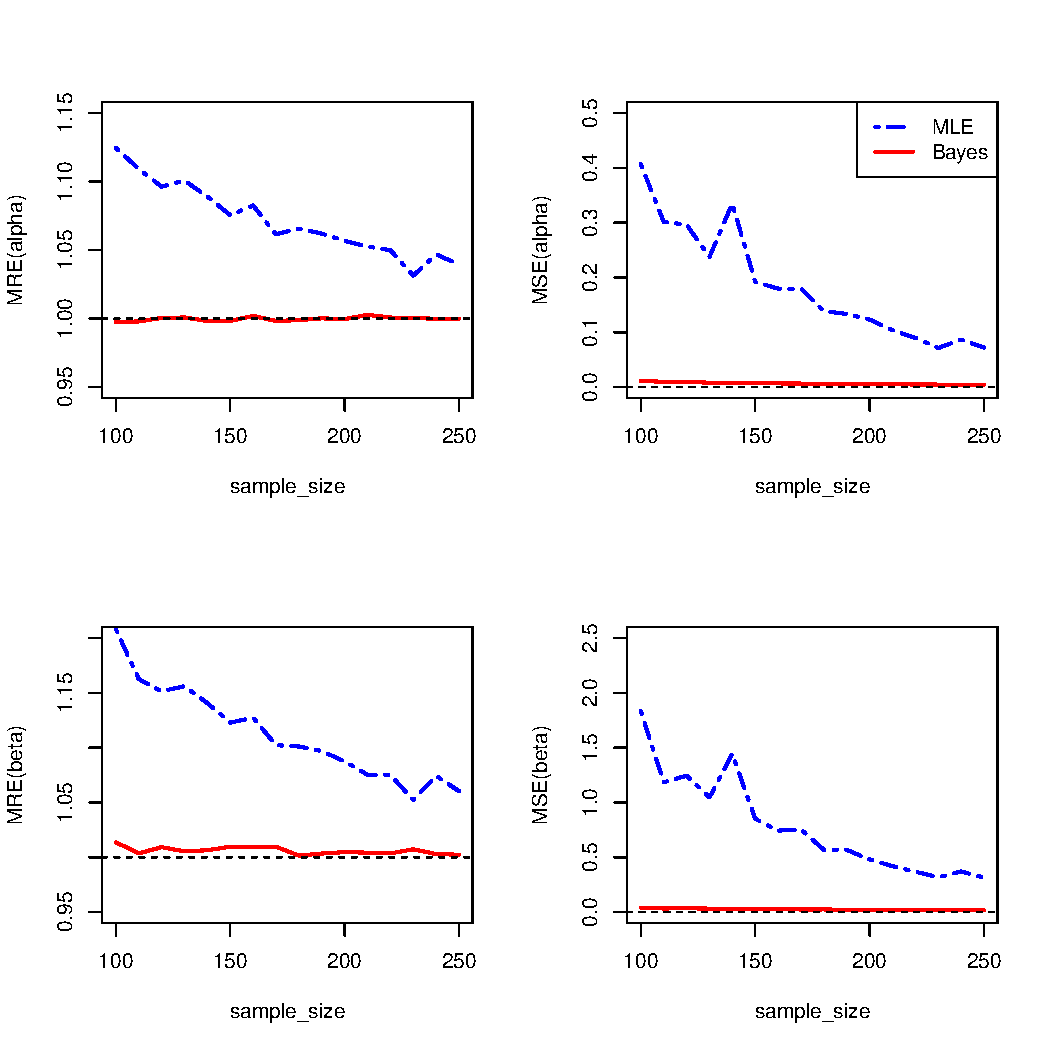
\includegraphics[width=55mm]{result}
\caption{シミュレーションの結果}
%\label{}
\end{center}
\end{figure}
\end{frame}



\begin{frame}
ベイズ推定は最尤推定よりも精度が優れているという結果になった. 
\end{frame}

\section{問題点と改善策の提案}
\begin{frame}
{\large 目次}
\tableofcontents[currentsection]
\end{frame}

\begin{frame}{問題点と改善策の提案}
先のシミュレーションにおいて$\lambda_{i}$を用いたが, これは未知のパラメータ$\alpha$に依存する分布からの確率変数であり, 通常これを得ることができない. 

これに対する改善案を二つ考え, シミュレーションを行なった. 
\end{frame}


\subsection{提案1}
\begin{frame}
まずは$\lambda_{i}$を用いずに事後分布を求める.

$\beta,\alpha$の同時事後分布は
$$
\pi(\beta ,\alpha |\bm{x})
\propto
\frac{\alpha^{n-1/2}\beta ^{-(n+1)}}{(\alpha +1)(\alpha +2)^{1/2}}
\prod_{i=1}^{n}
\left(1+\frac{x_{i}}{\beta }
\right)^{-(\alpha +1)}.
$$
これを用いて$2$変数のメトロポリス法により事後分布からの乱数を生成する. 
\end{frame}

\begin{frame}
\begin{figure}[ht]
\begin{center}
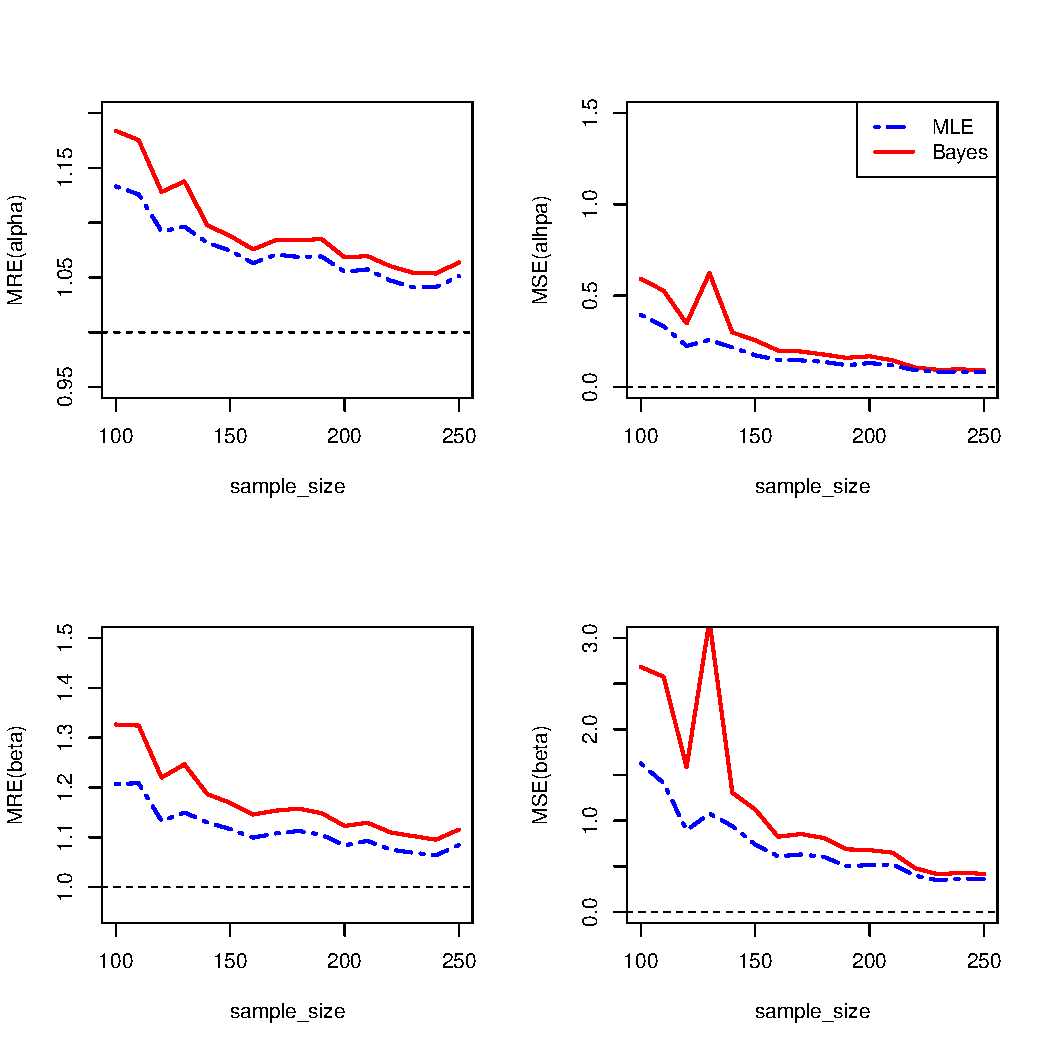
\includegraphics[width=55mm]{notlambda}
\caption{提案1のシミュレーションの結果}
%\label{}
\end{center}
\end{figure}
\end{frame}


\begin{frame}
提案$1$では$\lambda_{i}$を用いずに推定することができるが, 最尤推定と比べて精度が低下した. 
\end{frame}

\subsection{提案2}
\begin{frame}
次に$\lambda_{i}$を推定し, それを用いてパラメータ推定を行う.

$\lambda_{i}$の条件付き分布は

$$
\lambda _{i}|x_i,\beta ,\alpha 
\sim 
\mbox{Gamma} \left(\alpha +1,1+\frac{x_{i}}{\beta }\right)
$$
であった.
これを最尤推定値$\hat{\beta },~\hat{\alpha }$を用いて
$$
\lambda _{i}|x_i,\hat{\beta } ,\hat{\alpha } 
\sim 
\mbox{Gamma} \left(\hat{\alpha } +1,1+\frac{x_{i}}{\hat{\beta }}\right)
$$
として各$\lambda_i$を推定する.

\end{frame}


\begin{frame}
\begin{figure}[ht]
\begin{center}
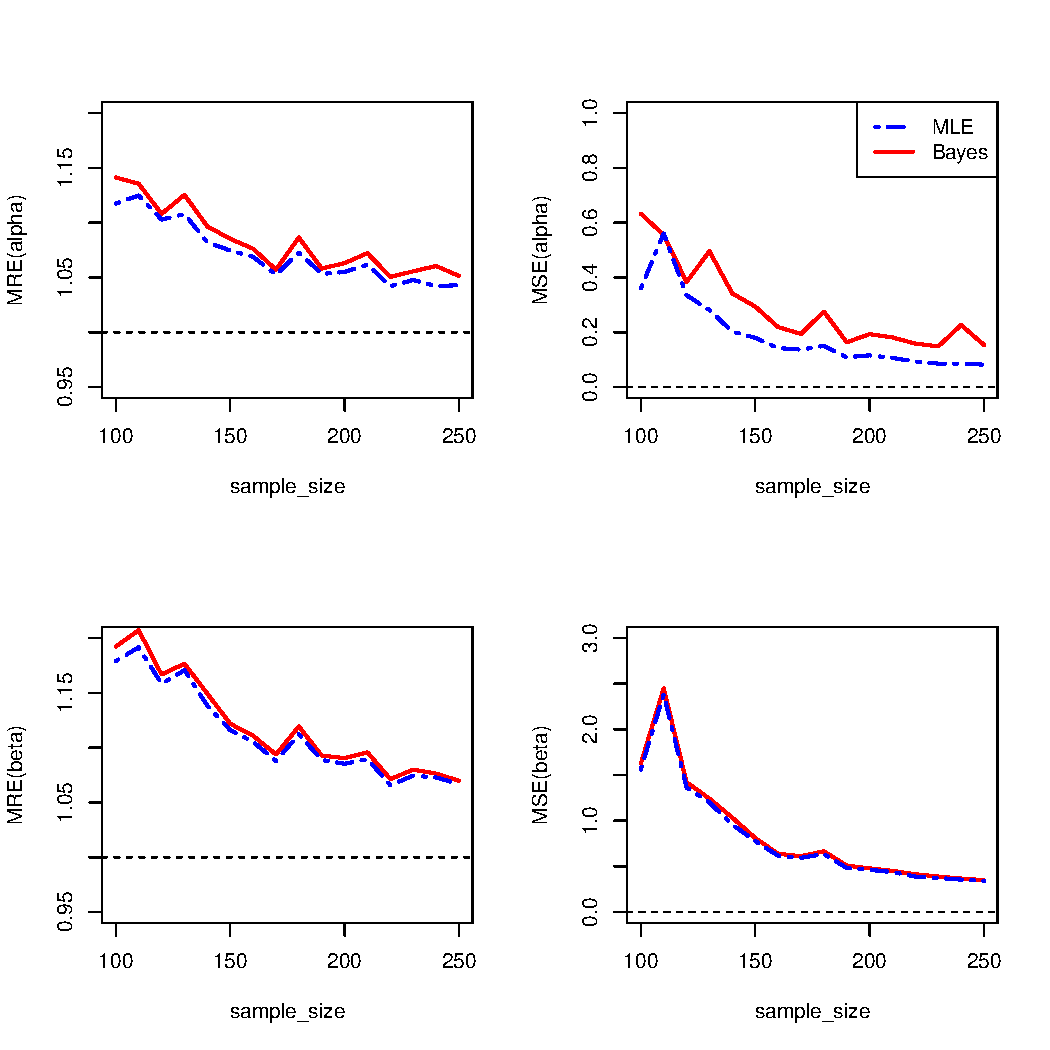
\includegraphics[width=55mm]{mle-bayes}
\caption{提案2のシミュレーションの結果}
%\label{}
\end{center}
\end{figure}
\end{frame}



\begin{frame}
提案$2$では$\lambda_{i}$が得られなくても推定が可能であるが, 提案$1$と同様に最尤推定と比べて精度が低下した. 
\end{frame}

\section{まとめ}


\begin{frame}
{\large 目次}
\tableofcontents[currentsection]
\end{frame}

\begin{frame}{まとめ}

\cite{Lomax2020}のシミュレーションの再現ではベイズ推定の方が精度が良いことが確認できたが, 問題点があり, それについて検討した. 

今回提案した二つの手法は現実的に用いることは可能であるが, 推定の精度は最尤推定より劣っていて, 実用的ではない. 

今後は$\lambda_i$を別の方法で生成, または$\lambda_i$を使わない方法によってより精度の高い推定法を考えることが課題である.

\end{frame}





\begin{frame}{参考文献}
\bibliographystyle{plain}
\bibliography{sample,jsample}
\end{frame}

\end{document}
